\section{Task II - Handover Vorhersage und Link Lifetime}


\begin{frame}{Datentransformation}
$\textbf{Idee}$: Prädiktionsmodell XGBoost für Link Lifetime mit Einfluss des \\
 \hspace{9mm} RSRP/RSRQ der verbundenen sowie der Nachbarzellen \\

\quad\\

$\rightarrow$ Datentransformation\\

\quad\\

	\begin{itemize}
		\item RSRP/RSRQ Nachbarzellen : \\
		$\rightarrow$ mehrere Messungen - Filtern des besten Wertes zum aktuellen \\
		\hspace{4mm} Zeitpunkt \\
		$\rightarrow$ keine Messungen - Übernehmen des letzten Wertes \\
		\item eNodeB Wechsel $\rightarrow$ Response Variable Link Lifetime
	\end{itemize} 
\end{frame}





\begin{frame}{Features}
	\begin{itemize}
		\item $\textbf{link\_lifetime}$ : Link-Lifetime
		\item $\textbf{rsrp\_dbm/rsrq\_db}$ : Signalstärke/Signalqualität (RSRP/RSRQ) der verbundenen Zellen
		\item $\textbf{rsrp\_neighbor/rsrq\_neighbor}$ : Signalstärke/Signalqualität (RSRP/RSRQ) der Nachbarzellen
		\item $\textbf{rssnr\_db}$ : Signal-Rausch-Verhältnis (RSSNR)
		\item $\textbf{eNodeB}$ : Funkmasten im LTE-Netzwerk
		\item $\textbf{velocity\_mps}$ : Geschwindigkeit des mobilen Endgeräts
		\item $\textbf{ta}$ : Timing Advance (TA) - Wert zur Synchronisation zwischen Up- und Downlink 
		\item $\textbf{cqi}$ : Channel Quality Indicator (CQI) 
	\end{itemize}
\end{frame}




\begin{frame}{Vorgehen}
Wichtige Schritte : 
	\begin{itemize}
		\item Aufsplitten der Daten - Training/ Test
		\item Zufälliger Grid-Search
		\item Tunen der Parameter - Zeitreihenkreuzvalidierung
		\item Validieren des Modells auf dem Testdatensatz 
	\end{itemize}

\quad\\


$\rightarrow$ $\textbf{Analog zu Task I}$
\end{frame}





\begin{frame}{Ergebnisse - Zeitreihenplot O2}
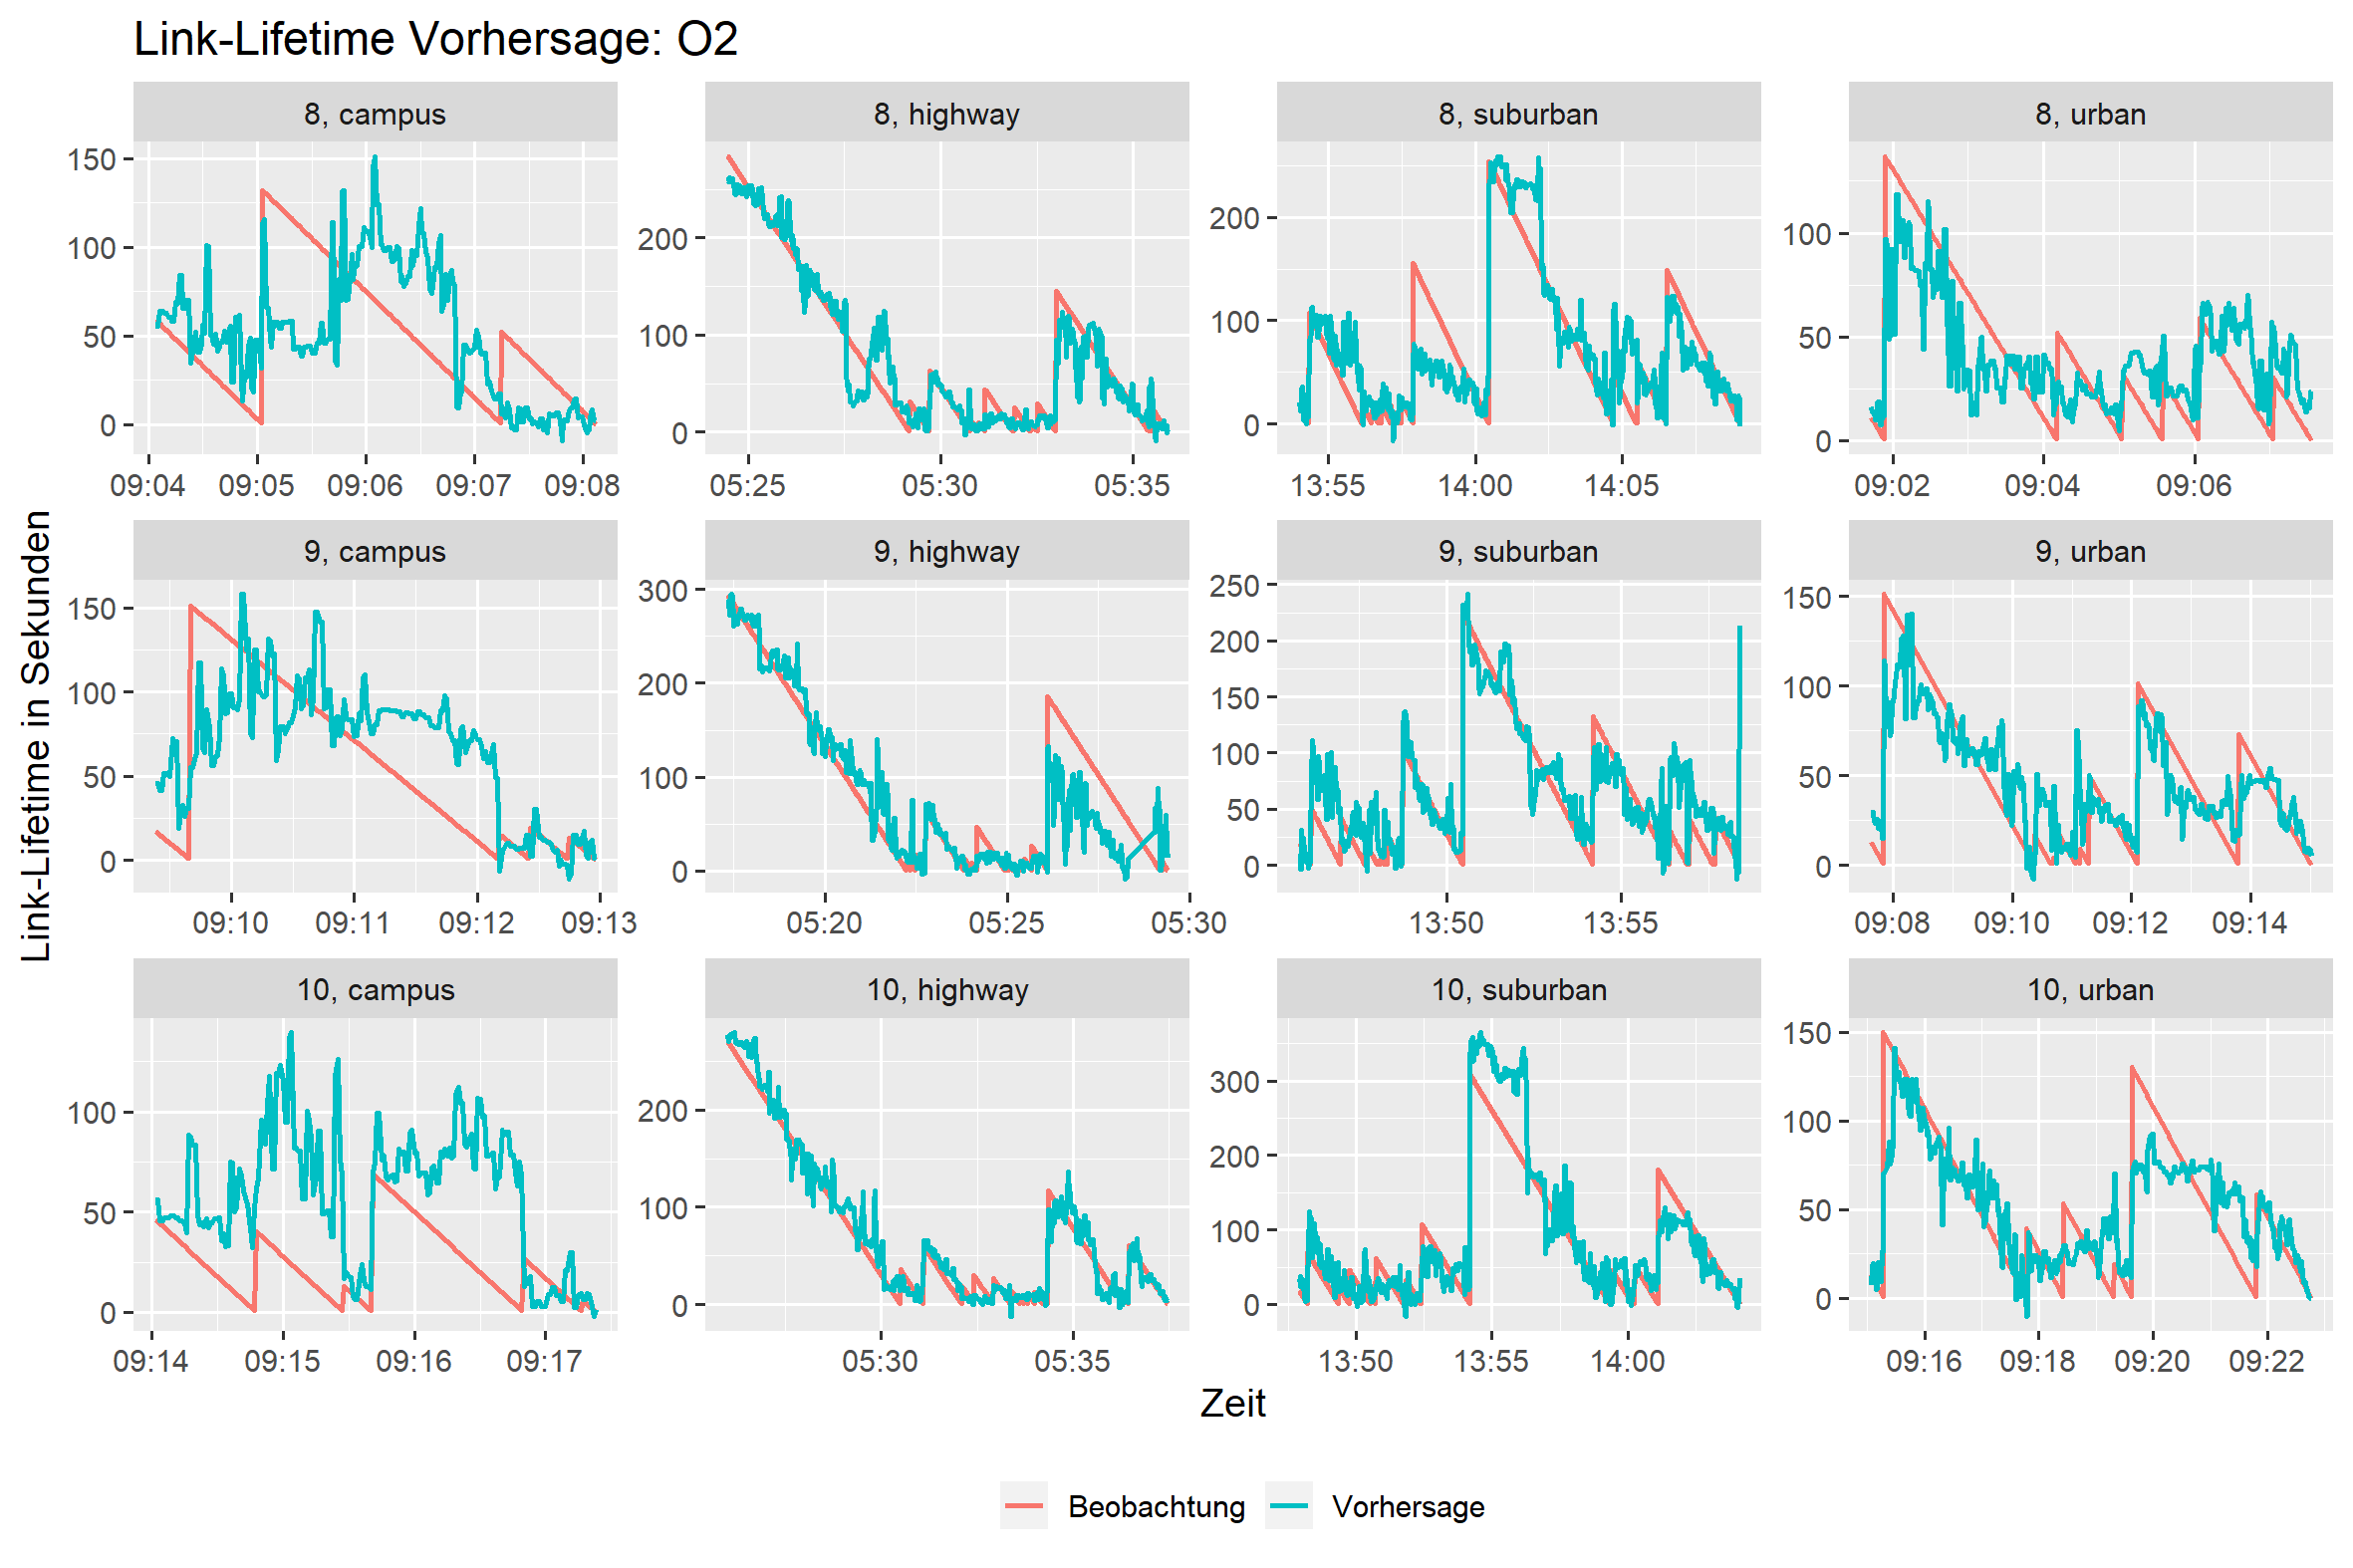
\includegraphics[width = 11cm]{plots/link_lifetime/o2_predictions}
\end{frame}


\begin{frame}{Ergebnisse - Zeitreihenplot T-Mobile}
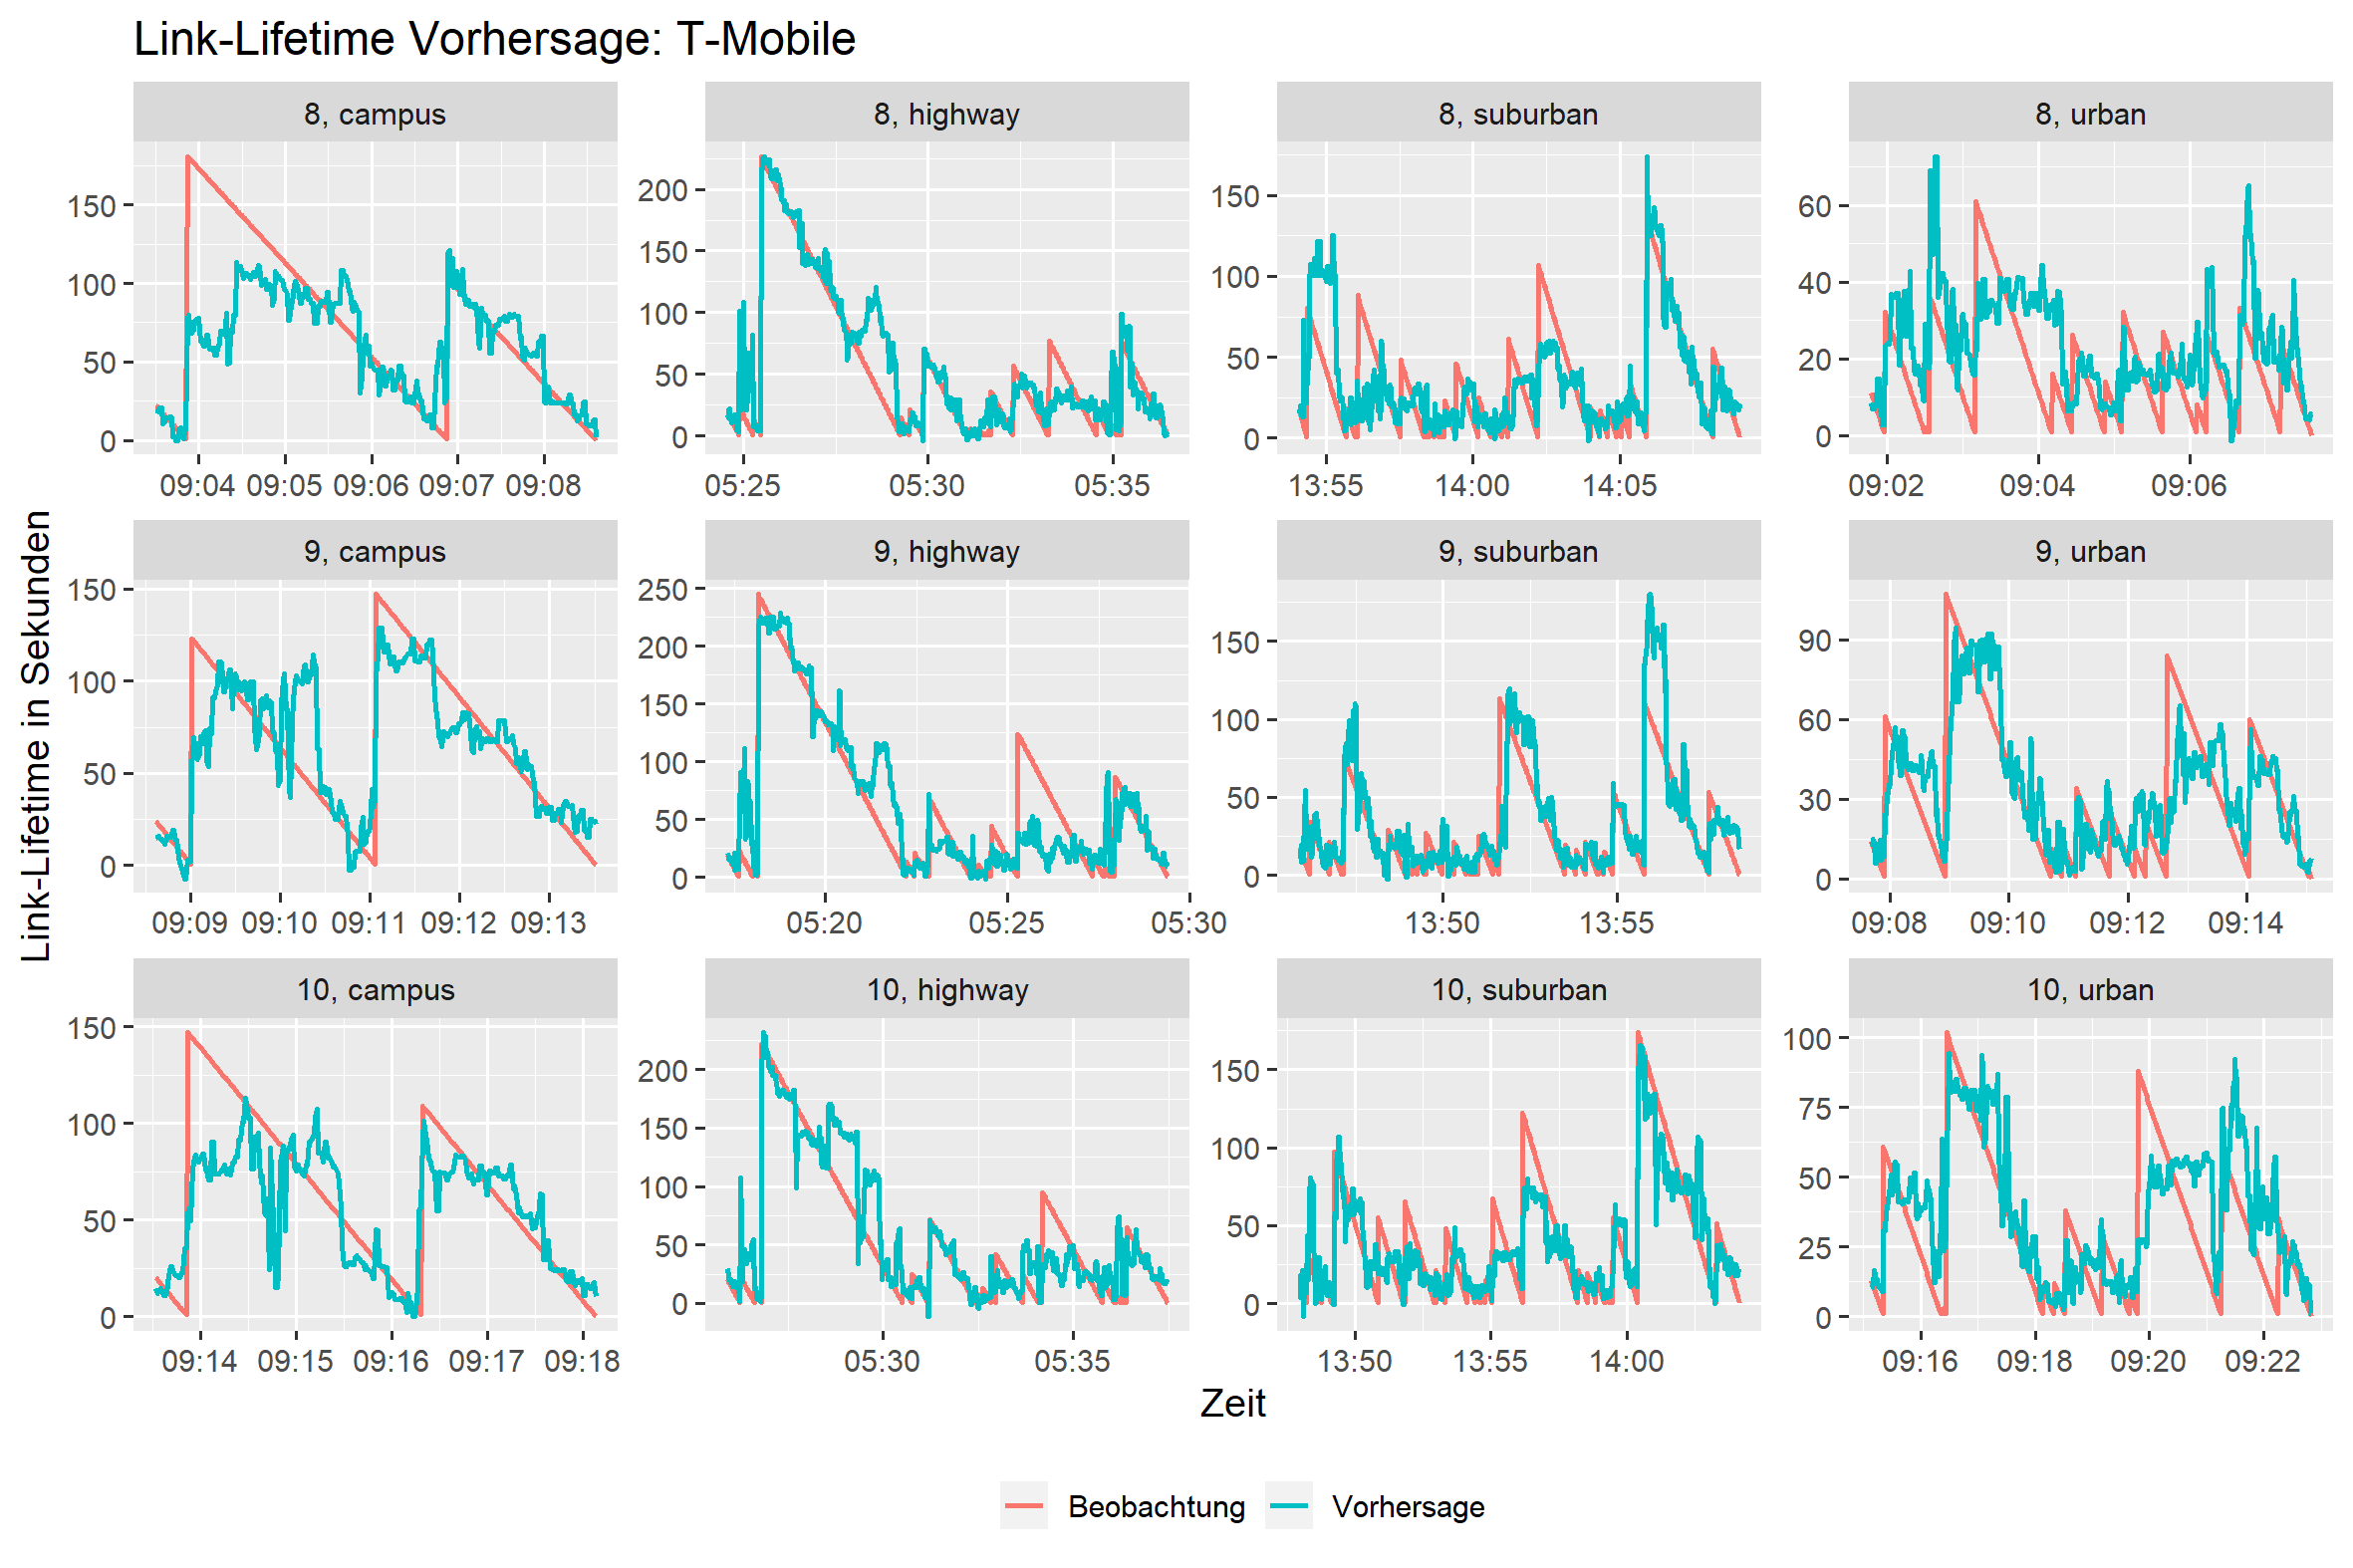
\includegraphics[width = 11cm]{plots/link_lifetime/tmobile_predictions}
\end{frame}


\begin{frame}{Ergebnisse - Zeitreihenplot Vodafone}
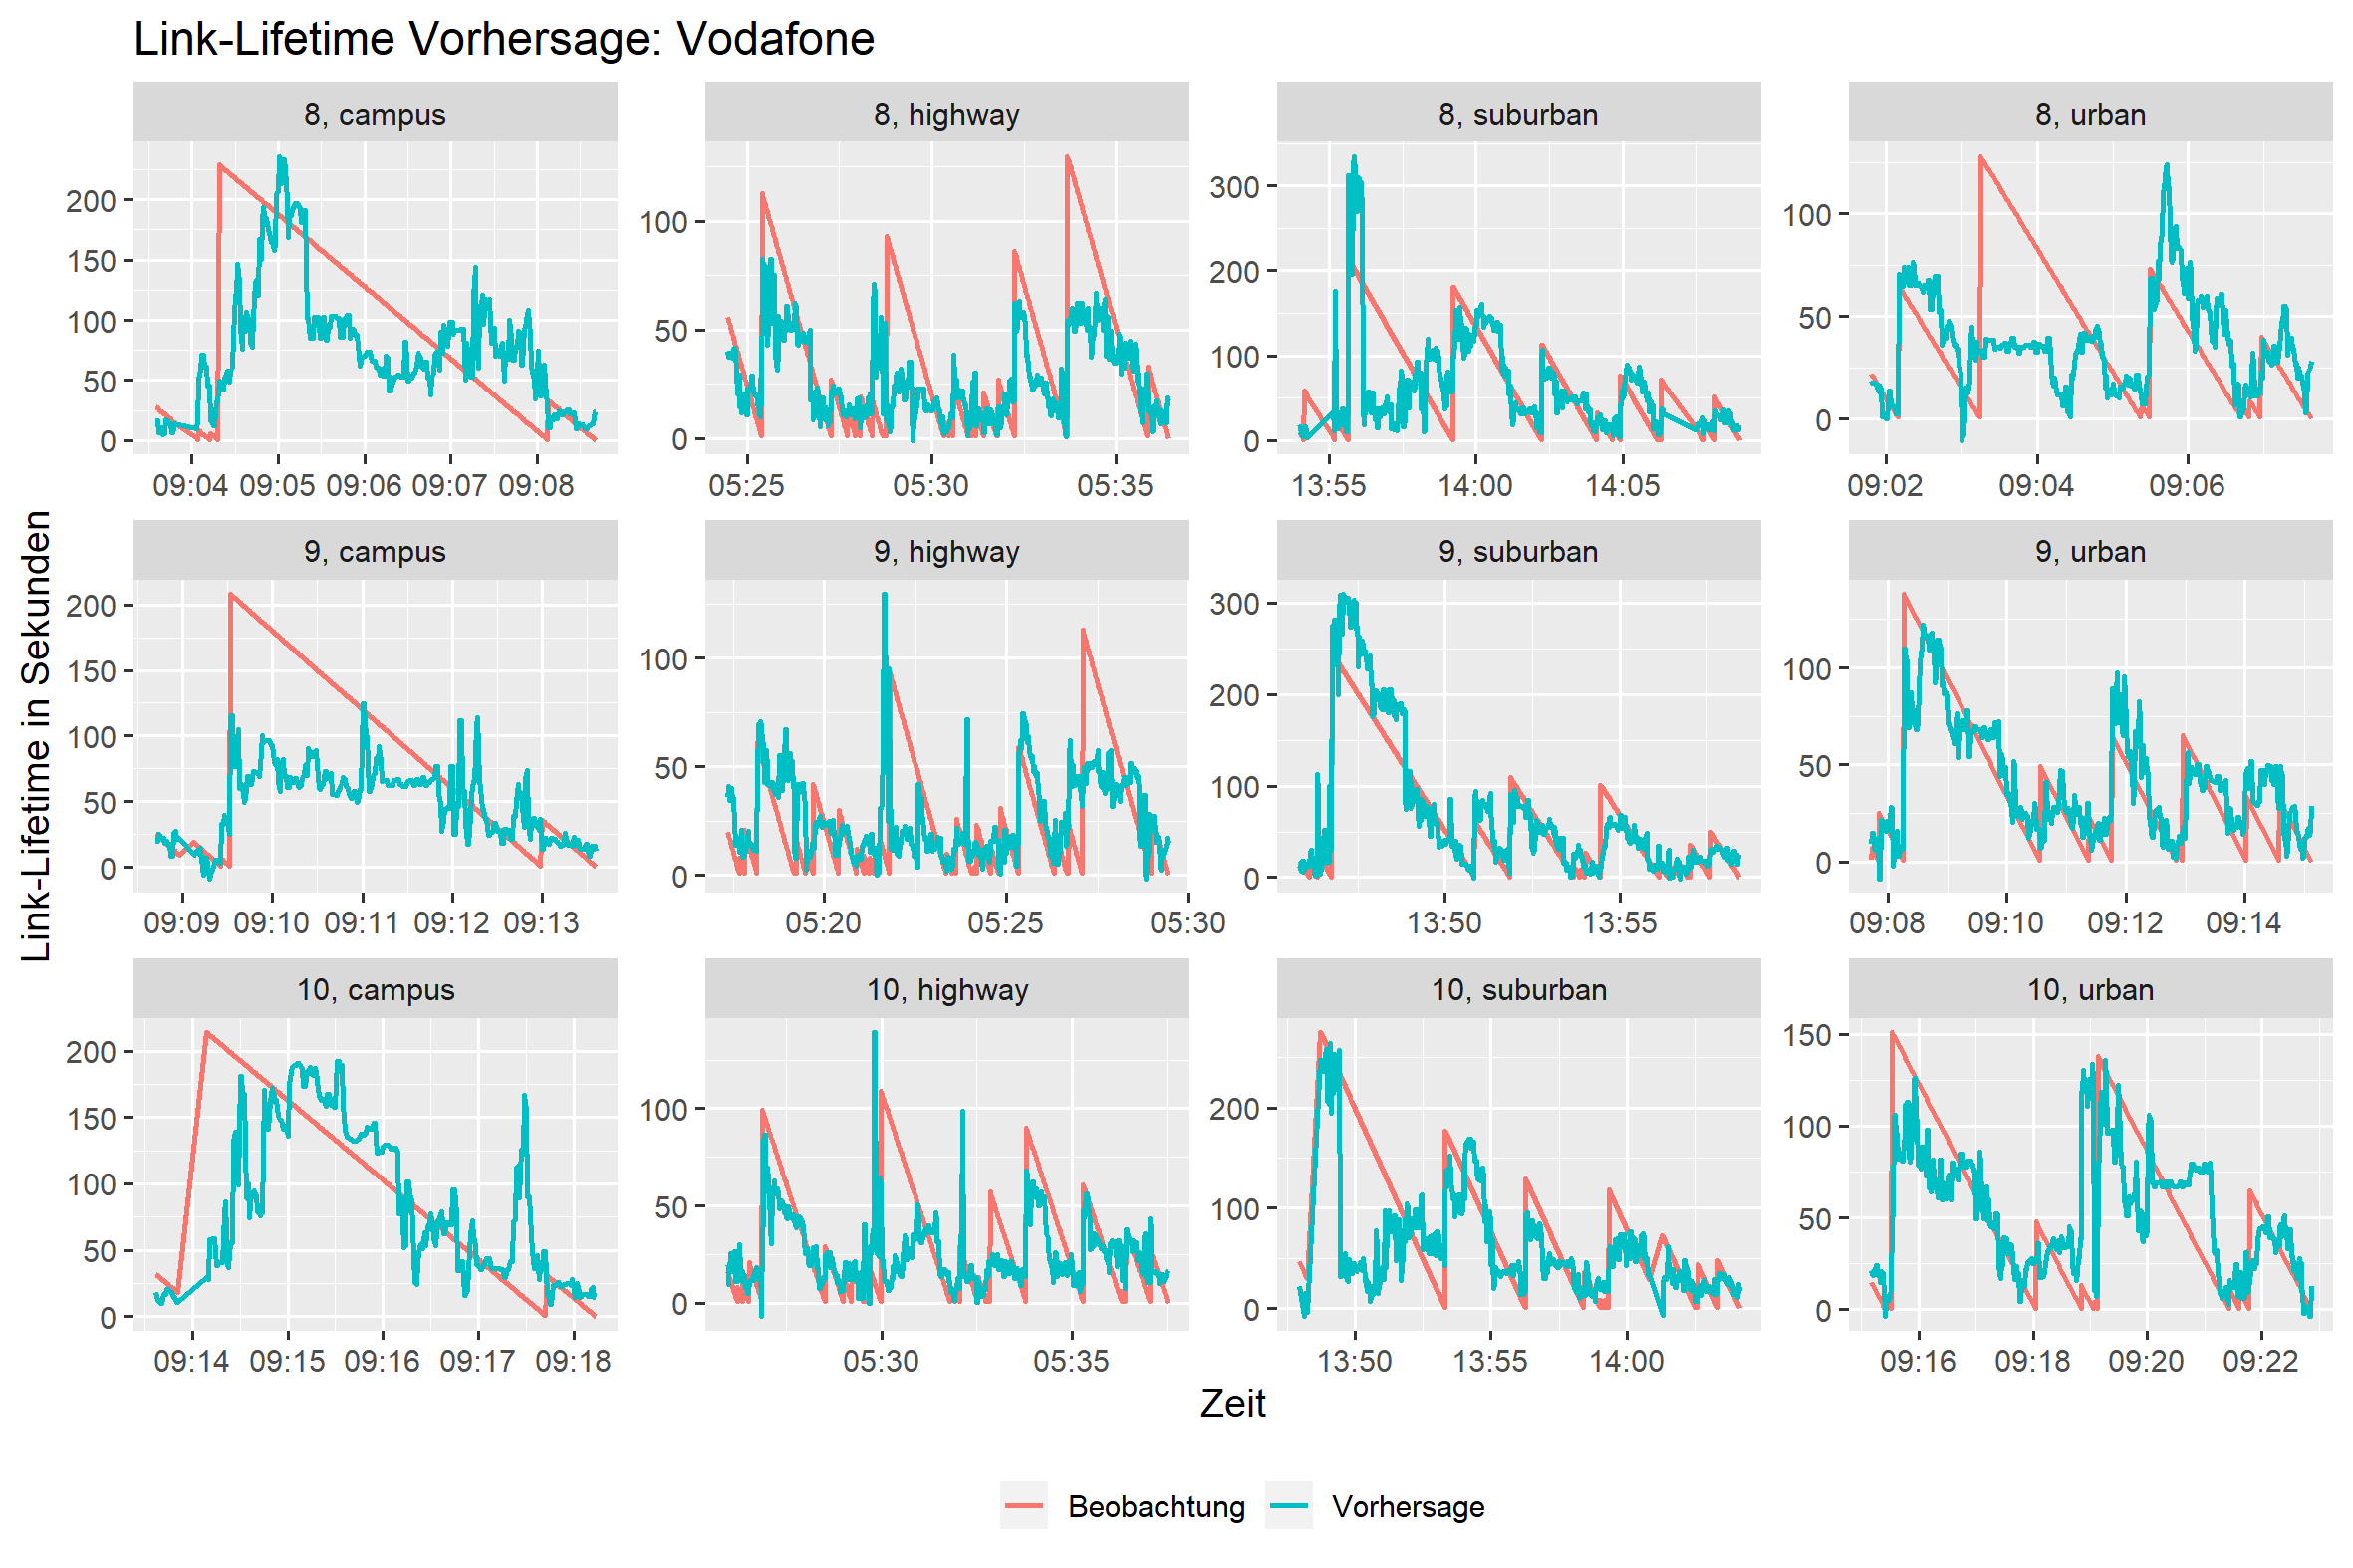
\includegraphics[width = 11cm]{plots/link_lifetime/vodafone_predictions}
\end{frame}


\begin{frame}{Ergebnisse - Scatterplot}
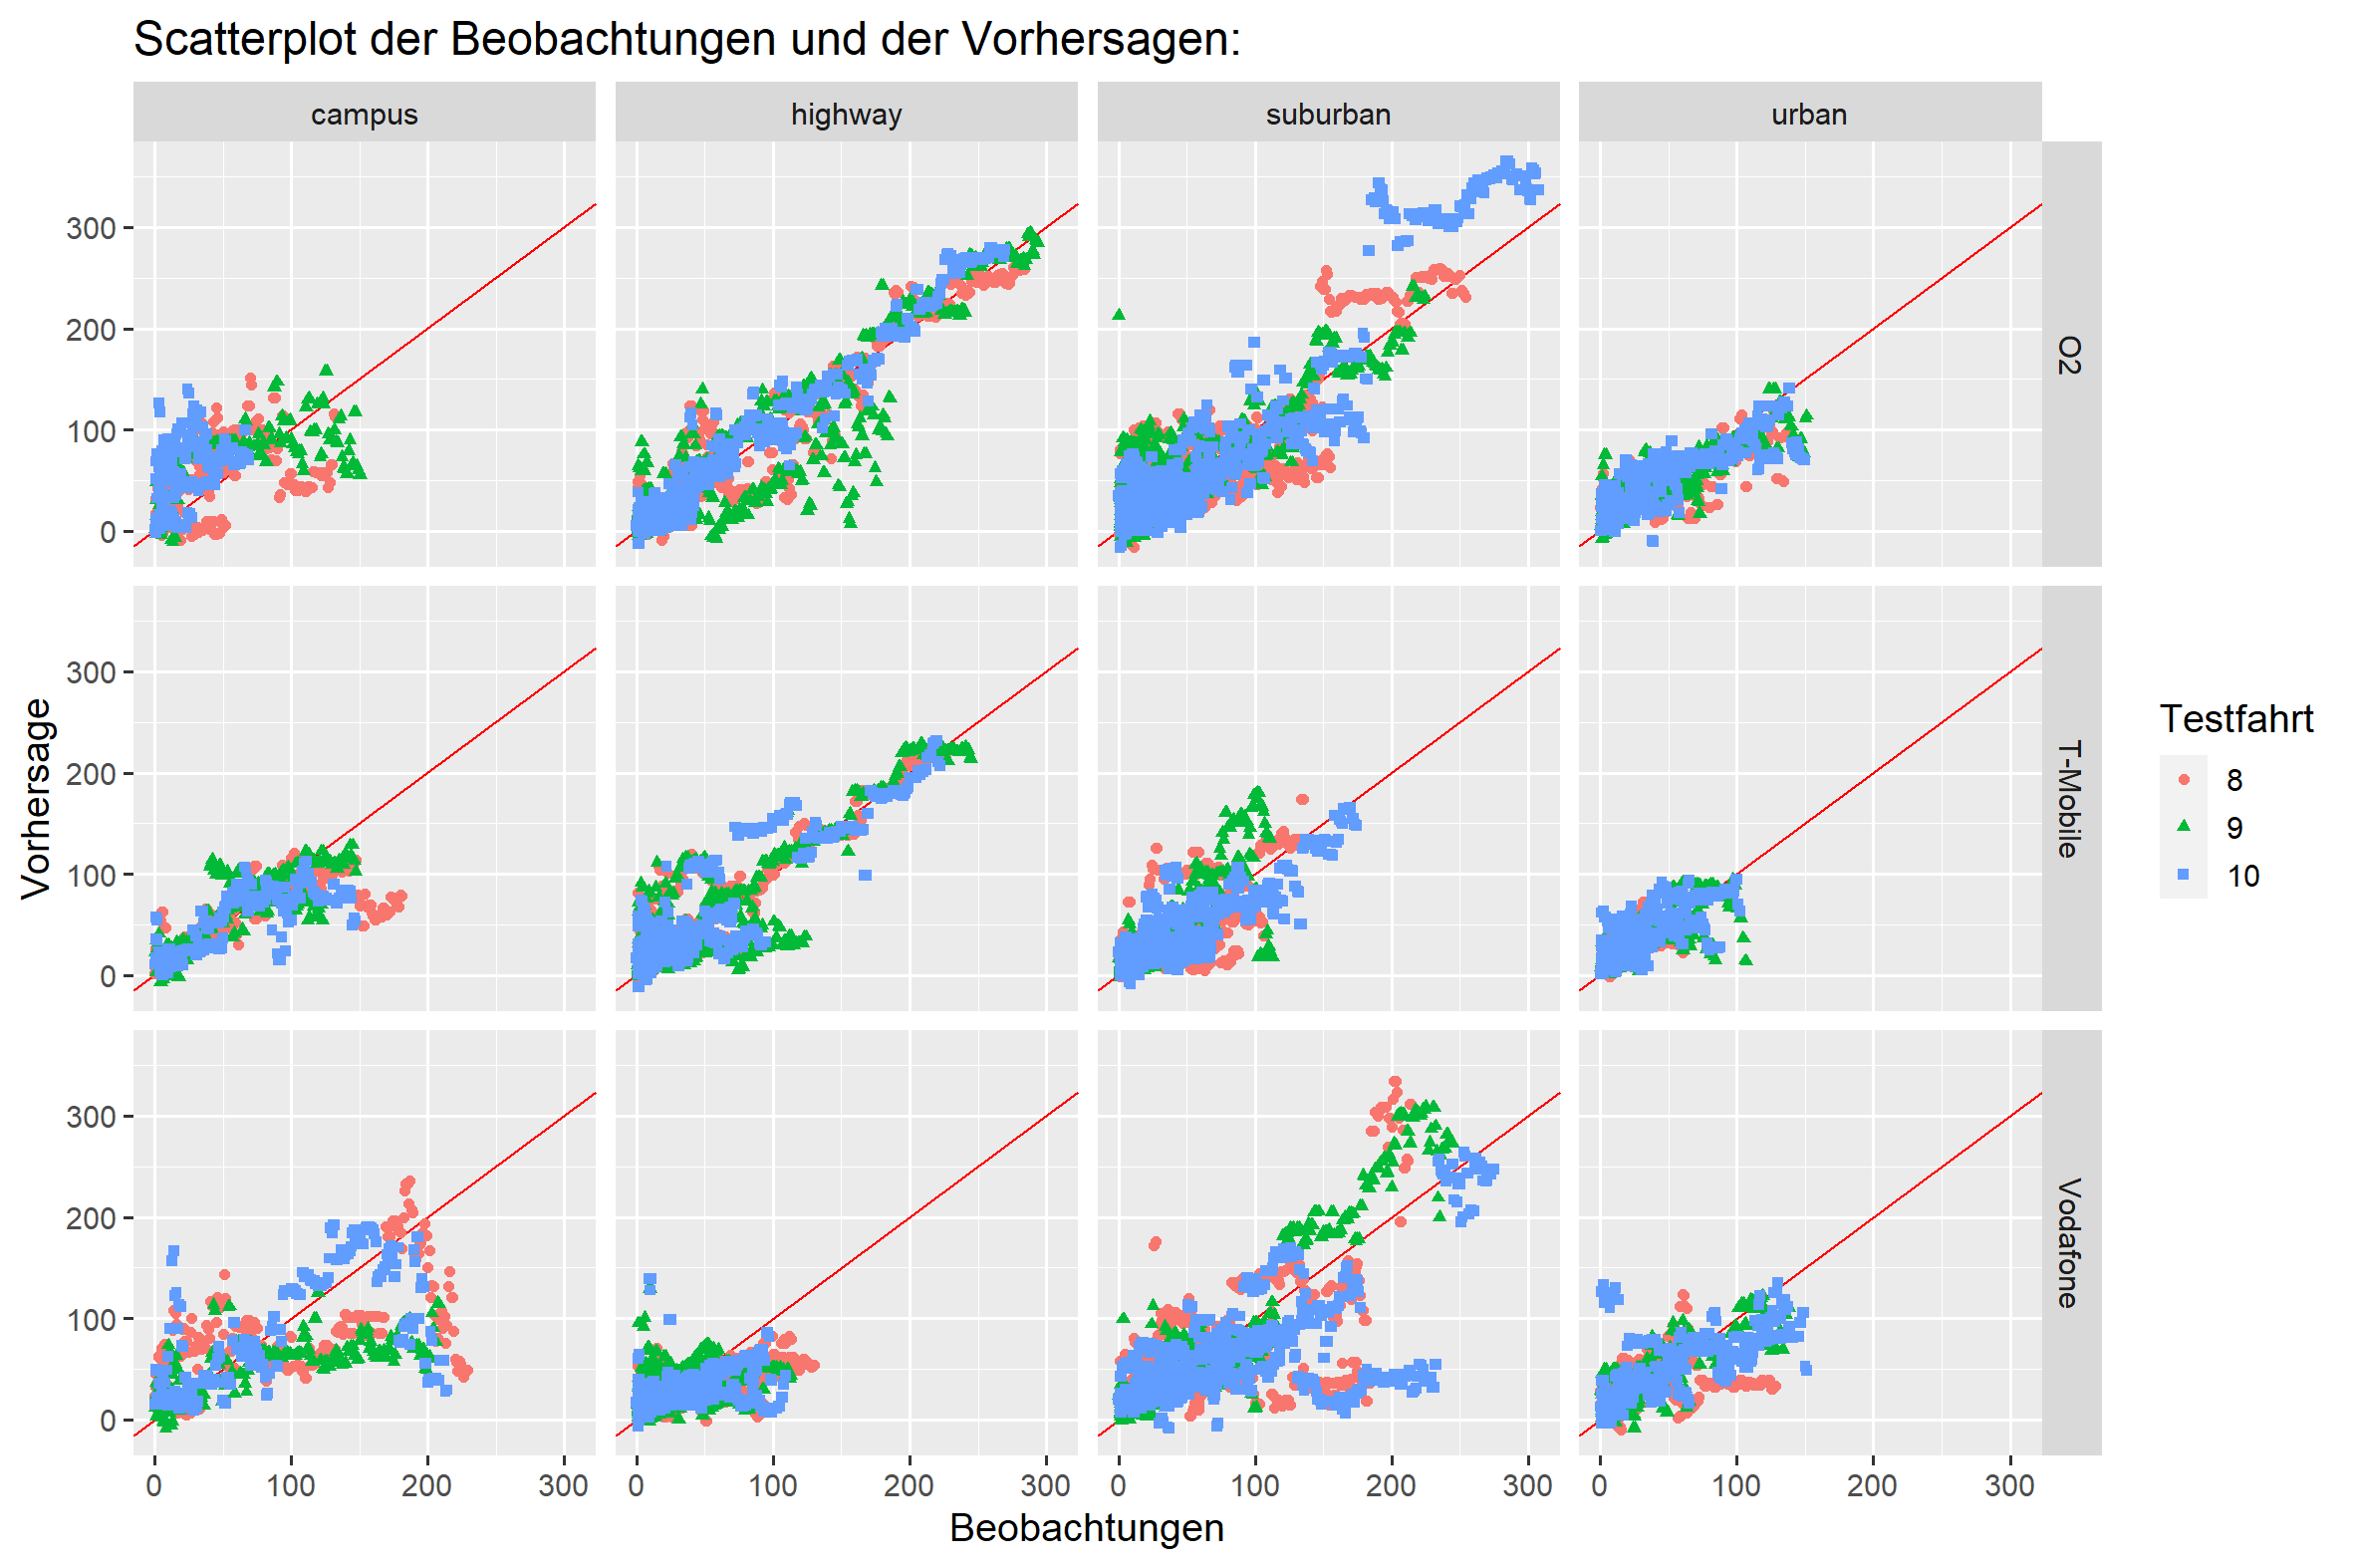
\includegraphics[width = 11cm]{plots/link_lifetime/scatter_colored_axes_fixed}
\end{frame}


\begin{frame}{Ergebnisse - Kennzahlen}
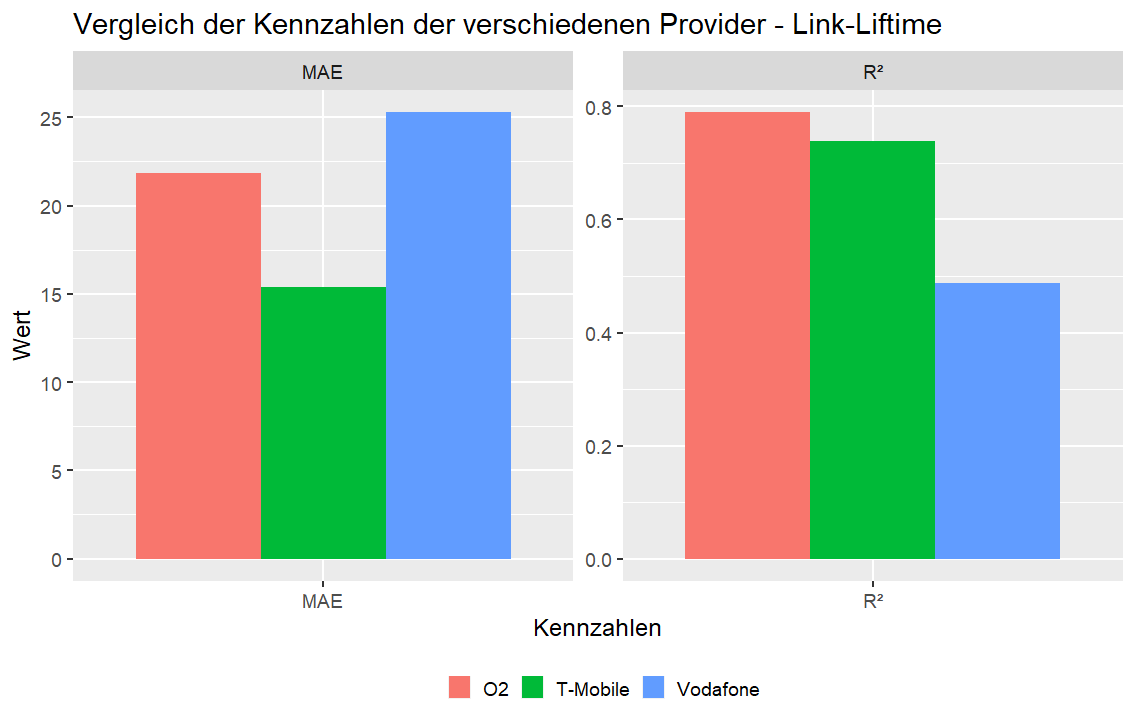
\includegraphics[width = 11cm]{plots/link_lifetime/kennzahlen_linklifetime}
\end{frame}

